
\section{Credibilidade baseada em Relacionamentos}
\label{sec::pg_cred_baseada_grafos}

Abordamos durante essa seção as métricas utilizadas como terminais dos indivíduos evoluídos para credibilidade baseada em relacionamentos, assim como descrito na Seção~\ref{subsec::individuos}. Todas as métricas contidas aqui são amplamente utilizadas em Redes Complexas (citacao), pois são medidas que conseguem explorar bem as propriedades estruturais dos grafos modelados.

Lembramos que o primeiro passo é a construção dos grafos representando o relacionamento modelado do ponto das várias classes. 
Como já dito, construímos um grafo para cada classe, de forma a efetivamente isolar um classe da outra.
Logo depois, introduzimos o exemplo de teste e todas suas arestas para os exemplos de treinamento. Assim, de forma geral, calculamos para cada uma das classe o valor da métrica, $\textsc{Métrica}(teste, classe)$, que modela a credibilidade de determinada classe em relação ao exemplo de teste. 

Várias métricas não relacionam diretamente o teste a uma classe, mas o teste a cada um dos exemplos de treinamento de uma classe. Esse é o caso das métricas de similaridade, como veremos a seguir. Para essas situações, calculamos o valor da mesma para todos os exemplos de uma mesma classe e somamos os resultados obtidos. Logo,
\begin{equation}
         \textsc{Métrica}(teste, c_j) =  \sum\limits_{treino \in c_j} \textsc{Métrica}(teste, treino),
\end{equation}
resultando em somente um valor para a credibilidade de uma classe em relação ao exemplo de teste.

\subsection{Métricas modeladas.}
\label{subsec::pg_metricas_grafos}

Se eu seguir o padrao das ultimas secoes, aqui devo colocar uma tabela mostrando as metricas que vao ser usadas, como Adj(x). Faco isso mesmo?! Acho que sim. Esperando apenas confirmacao.


%As métricas usadas para atributos textuais consistem em algumas variantes do \textsc{TFIDF}, métrica mais difundida entre as apresentadas. Na tabela~\ref{table::metricas_textuais} estão concentradas algumas expressões amplamente utilizadas nas métricas aqui listadas.

%\begin{table}[ht*]
%\centering
%\begin{tabular}{|c|c|}
%\toprule
%    \textbf{Expressão} & \textbf{Explicação} \\
%\midrule
%    $N$           & Número de documentos na base de treinamento. \tabularnewline \hline
%    $M$           & Número de classes da coleção. \tabularnewline \hline
%    $D$           & Número de termos da coleção. \tabularnewline \hline
%\bottomrule
%\end{tabular}
%\caption{Explicação das principais expressões utilizadas para definição das métricas para atributos textuais.}
%\label{table::metricas_textuais}
%\end{table}


%%%%%%%%%%%%%%%%%%%-------------------------------------------------------%%%%%%%%%%%%%%%%%%%%%%%%%%%%%%%%%%%%%%%%
\subsubsection{Tamanho da Vizinhança}
\label{subsubsection::neighborhoodsize}

Um vértice adjacente, ou seja, conectado por uma aresta é dito ser um vértice vizinho de primeira ordem. Na Figura~\ref{fig::vizinhos}, temos que os vértices 2, 3, 4 e 5 são vizinhos de primeira ordem do vértice 1. Seguindo esse raciocínio, o vértice 6 é vizinho de segunda ordem do vértice 1 e de terceira ordem do vértice 2 e 3. 
Simplesmente contar o número de vizinhos existentes, dada uma ordem de vizinhança, consiste na métrica mais simples que podemos utilizar para relacionar um vértice a um grafo. Um exemplo de teste com muitas ligações ao grafo de uma determinada classe tem mais chances de pertencer aquela classe do que um outro exemplo que tem pouca ou nenhuma aresta que o conecta àquele grafo. 

Repare que decidimos não levar em consideração a direção das arestas quando temos um grafo direcionado. Somente nos importamos com o número de conexões totais do teste ao grafo de uma determinada classe, independente de serem arestas de entrada ou de saída do vértice que representa o teste. Baseado nessa teoria, criamos 3 métricas relacionadas a vizinhança, denominadas \textsc{VizN(teste, classe)}, onde $N$ representa a ordem de vizinhaça do teste em determinada classe.

%Em um grafo direcionado, temos ainda a noção de direção de uma aresta, logo podemos ter uma aresta que aponta de um vértice A para um vértice B, mas não o contrário. Em um grafo de citações por exemplo, um documento A que cita um outro documento B, é representando como uma aresta de aponta do vértice A para vértice B. O número de vizinhos que um vértice tem é chamado grau do vértice. Temos ainda os conceitos de grau de entrada e de saída, representando o número de arestas que chegam e saem de um vértice, respectivamente. 

\begin{figure}[ht!]
\centering
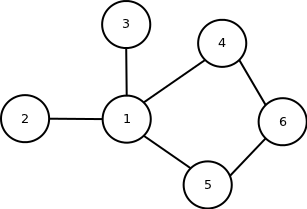
\includegraphics[width=0.4\textwidth]{figures/vizinhos.png}
\caption{A instância de teste triângulo está ligada ao grafo formado pela classe dos círculos e dos losangos, porém não apresenta ligações com os quadrados.}
\label{fig::vizinhos}
\end{figure}

%%%%%%%%%%%%%%%%%%%-------------------------------------------------------%%%%%%%%%%%%%%%%%%%%%%%%%%%%%%%%%%%%%%%%
\subsubsection{Força}
\label{subsubsection::strength}

A métrica \textsc{força(teste,classe)} é uma variação do tamanho da vizinhança de primeira ordem. Quando temos um grafo no qual as arestas têm peso, essa métrica realiza a soma dos pesos das arestas vizinhas ao invés de contar o número das mesmas. O peso de uma aresta, como já dito, é uma forma de representarmos informações importantes em relação aos vértices ligados pela aresta. Em um grafo em que os vértices representam cidades e as arestas representam ligações entre essas cidades, o peso de uma aresta pode significar a distância entre duas cidades, por exemplo. Dessa forma, pode ser mais significativo saber o quão longe (ou perto) uma cidade esta de suas vizinhas do que simplesmente saber o número de vizinhas que a mesma possui.
Destacamos que quando um grafo não possuí pesos nas arestas, atribuímos um peso unitário para todas as arestas, logo a \textsc{força} de um vértice seria igual ao grau de primeira ordem dele.

%%%%%%%%%%%%%%%%%%%-------------------------------------------------------%%%%%%%%%%%%%%%%%%%%%%%%%%%%%%%%%%%%%%%%
\subsubsection{Proximidade}
\label{subsubsection::closeness}

De maneira intuitiva, dizemos que dois objetos estão próximos se eles estão a uma distância arbitrariamente pequena um do outro. Muitas vezes, entretanto, não é fácil estipular o que vem a ser uma distância pequena. 

Em teoria dos grafos, medimos a distância entre os vértices utilizando o algoritmo conhecido como \textit{caminho mínimo}, que caso não leve em consideração o peso das arestas, conta o número mínimo de vértices que necessitamos atravessar para ligar conectar vértices escolhidos em um grafo. A \textsc{Proximidade(teste, classe)} (do inglês, \textit{Closeness}) é uma métrica que estima o quão próximo um vértice $v$ está em relação a todo o grafo usando a média dos caminhos mínimos de $v$ para todos os outros vértices alcançáveis a partir de $v$ (\cite{Beauchamp65}). Dessa forma, podemos medir a importância de um vértice calculando quanto tempo em média é gasto para uma informação se espalhar a partir de um vértice $v$ para todo o resto do grafo. Por fim, são considerados vértices mais ``próximos'' aqueles que minimizam esse tempo.

%%%%%%%%%%%%%%%%%%%-------------------------------------------------------%%%%%%%%%%%%%%%%%%%%%%%%%%%%%%%%%%%%%%%%
\subsubsection{Centralidade}
\label{subsubsection::constraint}
A métrica de centralidade (em inglês, \textit{Betweenness}) \textsc{Centralidade(teste, classe)} se baseia no fato que um vértice é importante em um grafo se ele está no percurso de outros vértices, sendo obrigatoriamente muito visitado. Sendo assim, um vértice tem maior credibilidade se for usado para conectar os vários vértices em um grafo, pertencendo a vários caminhos mínimos.
%Como já dito, o algoritmo do caminho mínimo é o que se utiliza para percorrer da melhor maneira possível uma dada distância em um grafo. 
A métrica \textsc{Centralidade} calcula a importância de um vértice contando quantas vezes aquele vértice participa do caminho mínimo entre quaisquer dois outros vértices do grafo em questão (\cite{Sabidussi66}). Obviamente, um vértice central que está no caminho mínimo de vários outros tem mais acesso a informação que circula pelo grafo que um vértice periférico com poucas ligações.

%%%%%%%%%%%%%%%%%%%-------------------------------------------------------%%%%%%%%%%%%%%%%%%%%%%%%%%%%%%%%%%%%%%%%
\subsubsection{Centralidade do Autovetor.}
\label{subsubsection::eigenvector}

A centralidade do Autovetor (\textsc{Eigen}(teste, classe), do inglês \textit{Eigenvector Centrality}) é uma medida de centralidade que avalia a importância de um vértice em todo o grafo. Ela atribui valores aos vértices baseados nas conexões que os mesmos têm, sendo que um vértice ganhará uma credibilidade maior se estiver conectado a vértices de maior credibilidade. Formalmente, dado que $x_i$ é o valor atribuído ao vértice $i$ e que podemos montar a matriz de adjacência $A$ com os $N$ vértices do grafo, na qual $A_{ij} = 1$ se existe uma aresta entre $i$ e $j$ e $A_{ij}=0$, caso contrário, temos:
\begin{equation}\label{eqn::eigenvector1}
   x_i = \frac{1}{\lambda} \cdot \sum\limits_{j=1}^{N} A_{ij} \cdot x_j
\end{equation}
Que pode ser reescrita utilizando vetores como:
\begin{equation}\label{eqn::eigenvector2}
   X = \frac{1}{\lambda} AX  \;\; \Longleftrightarrow\;\;  AX = \lambda X
\end{equation}
Onde $X$ é dito ser o \textit{autovetor} formado pelos valores de $x_i$ com $0 \leq i \leq N$ e associado ao \textit{autovalor} $\lambda$.  Podem existir muitos valores para $\lambda$ para os quais a Equação~\ref{eqn::eigenvector2} possui solução. Entretanto, se utilizarmos todos os valores do \textit{autovetor} como positivos, teremos o único e maior valor possível para o \textit{autovalor} (\cite{Newman10}). 

%%%%%%%%%%%%%%%%%%%-------------------------------------------------------%%%%%%%%%%%%%%%%%%%%%%%%%%%%%%%%%%%%%%%%
\subsubsection{\textit{Hub} e Autoridade de Kleinberg}
\label{subsubsection::hub}
As métricas conhecidas como \textsc{Hub(teste, classe)} e \textsc{Autoridade(teste, classe)} de Kleinberg são provenientes do trabalho de~\cite{Kleinberg99}. Elas também podem ser apresentadas em conjunto pelo nome de Algoritmo \textit{Hyperlink-Induced Topic Search} (HITS) e por serem predecessoras do \textit{PageRank}.

Em suma, a ideia aqui modelada se baseia no fato de que na \textit{Web}, algumas páginas são conhecidas como \textit{hubs} por não serem especialistas em nenhum assunto específico, mas possuírem ligações para vários outras páginas que são especialistas em seus respectivos assuntos, sendo, portanto, \textit{autoridades} no assunto tratado. Logo, o que temos é que um bom \textit{hub} é representado por uma página (vértice, no grafo que a \textit{Web} representa) que aponta para várias autoridades e uma boa autoridade é aquela apontada por vários \textit{hubs}. Uma página com poucas ligações e com poucas referências não é nem um bom \textit{hub} e nem uma boa autoridade.

%%%%%%%%%%%%%%%%%%%-------------------------------------------------------%%%%%%%%%%%%%%%%%%%%%%%%%%%%%%%%%%%%%%%%
\subsubsection{PageRank}
\label{subsubsection::pagerank}

O algoritmo \textit{PageRank} tem seu nome proveniente do seu criador Lawrence Page (\cite{Page98}). Assim como o algoritmo \textit{HITS}, Seção~\ref{subsubsection::hub}, o \textit{PageRank} se baseia na ideia de ordenar os vértices de um grafo baseado-se nas relações entre eles, sendo que quando mais ``popular'' um vértice é, maior é o seu \textit{PageRank}. Em resumo, temos que
\begin{equation}\label{eqn::pagerank}
PR(teste, classe) = \sum_{v \in Adj(a)} \frac{PR(v, classe)}{L(v)},
\end{equation}
onde $Adj(x)$ é o conjunto dos vizinhos do vértice $x$ e $L(x)$ é o grau de saída de $x$, ou seja, o número de vértices alcançáveis a partir de $x$.

%%%%%%%%%%%%%%%%%%%-------------------------------------------------------%%%%%%%%%%%%%%%%%%%%%%%%%%%%%%%%%%%%%%%%
\subsubsection{Burt's Constraint}
\label{subsubsection::constraint}

O termo capital social é um conceito sociológico abrangente, mas em geral pode-se dizer que está relacionado a relações sociais e consiste na expectativa de benefícios derivados de relações e cooperações entre indivíduos de um grupo e entre os vários grupos existentes na sociedade modelada. Ronald Burt é um sociologista que estudou alguns benefícios que indivíduos podem ter no mercado de trabalho provenientes das relações sociais que mantêm (\cite{Burt92}). Investigando as estruturas de rede do capital social, focando em indivíduos chaves em distintas organizações, ele chegou a conclusão que quem tem boas e diversificadas relações sociais consegue, entre outras coisas, melhores cargos, promoções e salários.  

Outro conceito importante são os buracos estruturais, que podem ser definidos como a falta de acesso entre sub-grafos distintos que compões um mesmo grafo. Burt propôs que vértices que conseguem preenche esses buracos estruturais, unindo vários sub-grafos, são mais importantes que aqueles vértices que estão unidos somente a um mesmo grafo ou os que estão isolados. Esse conceito é usado diretamente para calcular o~\textit{Burt's Constraint} de um vértice. Logo, \textsc{Burt}(teste, classe) é maior se o vértice de teste é capaz de se conectar a mais indivíduos que pertencem a partes não conectadas entre si do grafo modelado pela classe em questão.

%%%%%%%%%%%%%%%%%%%-------------------------------------------------------%%%%%%%%%%%%%%%%%%%%%%%%%%%%%%%%%%%%%%%%
\subsubsection{Bibliographic Coupling}
\label{subsubsection::bibcoup}
%http://igraph.sourceforge.net/doc/html/igraph_bibcoupling.html
\textit{Bibliographic Coupling} é uma métrica introduzida em~\cite{Kessler63} que calcula, para dois trabalhos científicos, o número de referências em comum que ambos possuem. A ideia dessa métrica é que se dois trabalhos apresentam muitas referências em comum, então provavelmente eles abordam o mesmo assunto. Em geral, podemos definir que:
\begin{equation}
\textsc{Bib}(a, b) =  |Adj(a) \cap Adj(b)|,
\end{equation}
onde $Adj(x)$ é o conjunto de vizinhos que o vértice $x$ está conectado. Como estamos interessados em calcular a similaridade de um vértice (exemplo de teste) com uma classe, necessitamos apenas de um valor que defina o quanto aquele vértice se assemelha aos demais. Logo, calculamos o valor do \textit{bibliographic coupling} do exemplo de teste com todos os vértices que ele se conecta:
\begin{equation}
\textsc{BibCoup}(teste, c_j) =  \sum\limits_{v' \in c_j} Bib(teste, v').
\end{equation}

%%%%%%%%%%%%%%%%%%%-------------------------------------------------------%%%%%%%%%%%%%%%%%%%%%%%%%%%%%%%%%%%%%%%%
\subsubsection{Co-Citação}
\label{subsubsection::cocitation}
A métrica co-citação mede, para dois vértices, o número de outros vértices que citam ambos (\cite{Small73}). Assim como a métrica \textit{Bibliographic Coupling}, procuramos atribuir um valor único para um exemplo de teste e, portanto, calculamos o somatório da co-citação entre o teste e todos os vértices presentes no grafo.
%TODO: se eu mudar para um unico grafo de varias classes, tenho que colocar aqui q to levando em consideracao so uma classe por vez.

%%%%%%%%%%%%%%%%%%%-------------------------------------------------------%%%%%%%%%%%%%%%%%%%%%%%%%%%%%%%%%%%%%%%%
\subsubsection{Similaridade de Jaccard}
\label{subsubsection::jaccard}

A similaridade de Jaccard, ver~\cite{Jaccard01}, é uma métrica muito antiga que pode ser definida como o tamanho da interseção de dois conjuntos divididos pela união dos mesmos. Podemos definir a similaridade de Jaccard matematicamente como:
\begin{equation}
\textsc{Jac}(a, b) =  \frac{|Adj(a) \cap Adj(b)|}{|Adj(a) \cup Adj(b)|},
\end{equation}
e da mesma forma que já realizado anteriormente, calculamos o somatório dessa métrica entre o exemplo de teste e todos os vértices do grafo.


%%%%%%%%%%%%%%%%%%%-------------------------------------------------------%%%%%%%%%%%%%%%%%%%%%%%%%%%%%%%%%%%%%%%%
\subsubsection{Similaridade de Dice}
\label{subsubsection::dice}

O coeficiente de similaridade de Dice de dois vértices é duas vezes o número de vizinhos em comum dividido pela soma de graus dos dois vértices, ver~\cite{Dice45}. Matematicamente temos:
\begin{equation}
\textsc{Dice(a,b)} = \frac{2 \cdot | adj(a) \cap adj(b) | }{| a | + | b |},
\end{equation}
onde $adj(x)$ é o conjunto de vértices adjacentes ao vértice $x$. Novamente, calculamos a similaridade de Dice entre o exemplo de teste e todos os vértices do grafo, a fim de termos um único valor que represente a credibilidade do ponto de vista dessa métrica.

%%%%%%%%%%%%%%%%%%%-------------------------------------------------------%%%%%%%%%%%%%%%%%%%%%%%%%%%%%%%%%%%%%%%%
\subsubsection{ Similaridade de Adamic e Adar}
\label{subsubsection::inverselog}

As similaridades de Jaccard e Dice se baseiam no princípio que todos os vértices adjacentes ao vértice que analisamos são igualmente importantes. Entretanto, esse não é sempre o caso.
Inspirados em uma ideia similar ao TDIDF, Seção~\ref{subsubsection::tfidf}, Adamic e Adar propuseram atribuir pesos aos vértices de maneira que um vértice com menos conexões possa ter maior poder discriminativo, ver~\cite{Adamic03}. Dessa forma, a similaridade de Adamic e Adar entre dois vértices é o número de vizinhos que ambos têm em comum, balanceados pelo inverso do logaritmo de seus graus. Ou seja,
\begin{equation}
\textsc{Ad\&Ad(a,b)} =  \sum\limits_{v \in (adj(a)\ \cap\ adj(b))} \frac{1}{ \log(dg(v))},
\end{equation}
onde $dg(g)$ é grau do vértice $v$ e $adj(x)$ é o conjunto de todos os vértices adjacentes de $x$. Como já dito, por fim necessitamos calcular o valor de \textsc{Ad\&Ad(teste, classe)} realizando o somatório da similaridade entre o teste e todos os vértices do grafo da classe em questão.


%\subsubsection{getAvgNearstNeighborDegree(id, className, graphId)}
%\label{subsubsection::avgnearst}
%acho que nao to uando


